	
	\section{Présentation UEDF}
	
	Nous avons déjà présenté précédemment \textbf{UEDF}, de façon globale et succincte. 
	Dans cette partie, nous allons détailler l'algorithme afin d'en avoir une meilleure compréhension. Cela 
	permettra de mesurer la différence entre les attentes théoriques et les résultats obtenus.\newline

	Nous avons évoqué les intérêts de l'implémentation d'\textbf{UEDF} :\\
	Tout d'abord, il est principalement \hyperref[inline]{en ligne}, ce qui n'est pas le cas de 
	la plupart des ordonnanceurs utilisés dans l'industrie.
	Ensuite, il est global. Or, la plupart des ordonnanceurs 
	globaux connus et implémentés ne sont pas optimaux (pour la classe périodique), pour la
	raison exposée au préalable dans ce travail : il est nécessaire d'avoir de la clairvoyance, 
	c'est à dire une connaissance relative du futur.\newline
	
	\todo{etat de l'art, parler de généralisation horizontale/verticale}
	
	\subsection{Définitions}
	Dans un premier temps, nous posons quelques définitions qui sont nécessaires à la compréhension de l'algorithme. 
	Par ailleurs, par souci de clarté, nous simplifions les calculs en supposant que les offsets [\ref*{offset}] des tâches 
	sont nuls dans la partie qui suit, cela ne change pas l'algorithme mais rend les explications moins 
	complexes.\\
	\subsubsection{Tâche active}\label{tacheactive}
	Ce qui définit une tâche \og{}active\fg{} peut différer selon le contexte. Dans l'approche d'\textbf{UEDF}, une tâche est 
	considérée comme active si un travail a été relâché et que ce travail n'a pas encore atteint son échéance. 
	Un travail $\tau_i$ est actif s'il a été relâché sur ou avant $t$ et que $d_i(t) \geq t$.
	Une tâche peut donc 
	être considérée comme active même si l'exécution d'un travail en cours est terminée. 
	Concrètement, si une tâche est périodique à échéance implicite [\hyperref[echeancesurrequete]{\ref*{echeancesurrequete}}], elle est active en permanence dès le 
	premier relâchement de travail. Le travail sera actif durant son relâchement jusqu'à ce que $t \geq d_i(t)$, où 
	une nouvelle instance de la tâche $\tau_i$ sera relâchée.
	
	
	\subsubsection{Ensemble des tâches actives}\label{ensembledestachesactives}
	Dans \textbf{UEDF}, on effectue le parcours d'une liste des tâches actuellement actives dans le système, 
	cette liste étant ordonnée par échéances. 
	 L'ensemble des tâches actives est écrit $A(t)$ dans les formules qui suivent.\newline
	
	Pour décrire \textbf{UEDF}, nous allons le décomposer en étapes.
	À chaque fois qu'un nouveau travail est relâché, cela va provoquer le calcul d'$Allot$.
	\subsubsection{Allot}
	Les tâches actives [\ref*{tacheactive}] sont ordonnées dans une liste. La priorité est définie selon l'échéance, 
	la plus petite étant la plus prioritaire, comme dans \textbf{EDF} [\ref*{EDF}].
	Dans cette phase, l'algorithme va \og{}réserver\fg{} des tranches de temps d'exécution des tâches sur les 
	processeurs, cela en calculant une valeur : \\
	$allot_{ij}$ pour $i \in \{0, nb\_de\_taches - 1\}$, pour $j \in \{0, nb\_processeurs - 1\}$
	La valeur $allot_{ij}$ représente le nombre d'unités d'exécution de la tâche $i$ réservé sur le processeur $j$.\newline
	Si cette valeur est positive, alors le temps $allot_{ij}$ du travail $i$ est réservé sur le 
	processeur $j$. Si cette valeur est égale à $0$, aucun temps n'est réservé 
	à l'exécution de la tâche $\tau_i$ sur le processeur $\pi_j$. Cela permet la constitution d'une liste, 
	\textbf{Eligible}.\newline


	Les calculs sont longuement décrits et expliqués dans la thèse de G. Nelissen \cite{nelissen_u-edf_2012}, aussi nous invitons 
	le lecteur curieux à se référer à ce document pour de plus amples détails. Mais en résumé, 
	ce calcul se déroule de cette façon :
	
	Nous posons :
	\begin{itemize}
		\setlength\itemsep{0.1em}
		\item $delay = d_i(t) - t$
		\item $ret_i = wcet - $ le nombre d'unités de temps déjà exécutées
		\item $m = $ le nombre de processeurs
		\item L'opérateur $[x]_a^b \defeq \max\{a, \min\{b, x \}\}$
	\end{itemize}


	\label{algouedf}
	\begin{algorithm}[H]
		\caption{Compute Allot}
		\begin{algorithmic}
			\REQUIRE $A(t)$ ordonné par échéances
			\STATE $W = 0$
			
			\FORALL{ $j \leftarrow \{1 ...m\} $}
				\item $RES_j \leftarrow 0$
				\item $ALLOT_j \leftarrow 0$
			\ENDFOR
	
			\FORALL{ $\tau_i \in A(t) $}
				\item $prev_i \leftarrow 0$
				\FORALL{ $j \leftarrow \{1 ...m\} $}
					\item $RES_j \leftarrow RES_j = \{[W]_{j-1}^{j} - (j - 1)\}\times (d_i(t) - d_{i-1}(t))$
					\item $ALLOT_{max} \leftarrow delay - ALLOT_j - RES_j - prev_i$
					\item $allot_{ij} \leftarrow min\{allot_{max}, ret_i - prev_i\}$
					\item $prev_i \leftarrow prev_i + allot_{ij}$
					\item $ALLOT_j \leftarrow ALLOT_j + allot_{ij}$
				\ENDFOR
				\item $W \leftarrow W + U_i$
			\ENDFOR
		\end{algorithmic}
	\end{algorithm}
	
	Dans l'exemple qui suit, notre système est composé de deux tâches :
	\begin{enumerate}
		\setlength\itemsep{0.1em}
		\item $\tau_1 : \{o:0; w:30; d=p:60;\}$
		\item $\tau_2 : \{o:0; w:60; d=p:80;\}$
	\end{enumerate}
	\begin{figure}[H]
		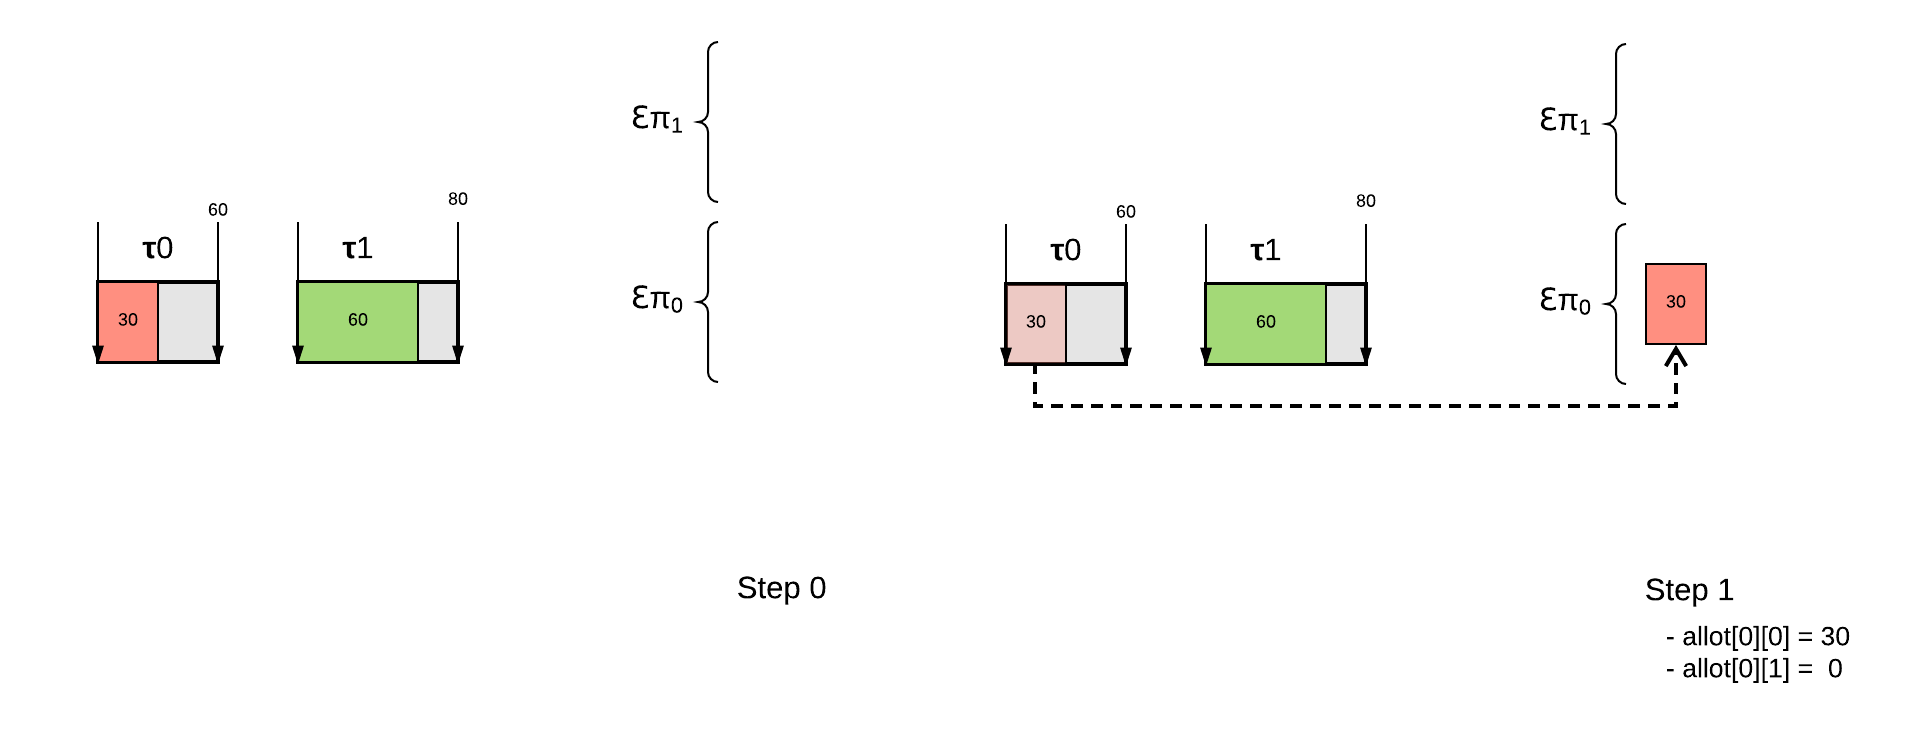
\includegraphics[scale=1]{img/uedf/uedf12}
		\caption{étapes 0 et 1}
	\end{figure}
	\begin{figure}[H]
		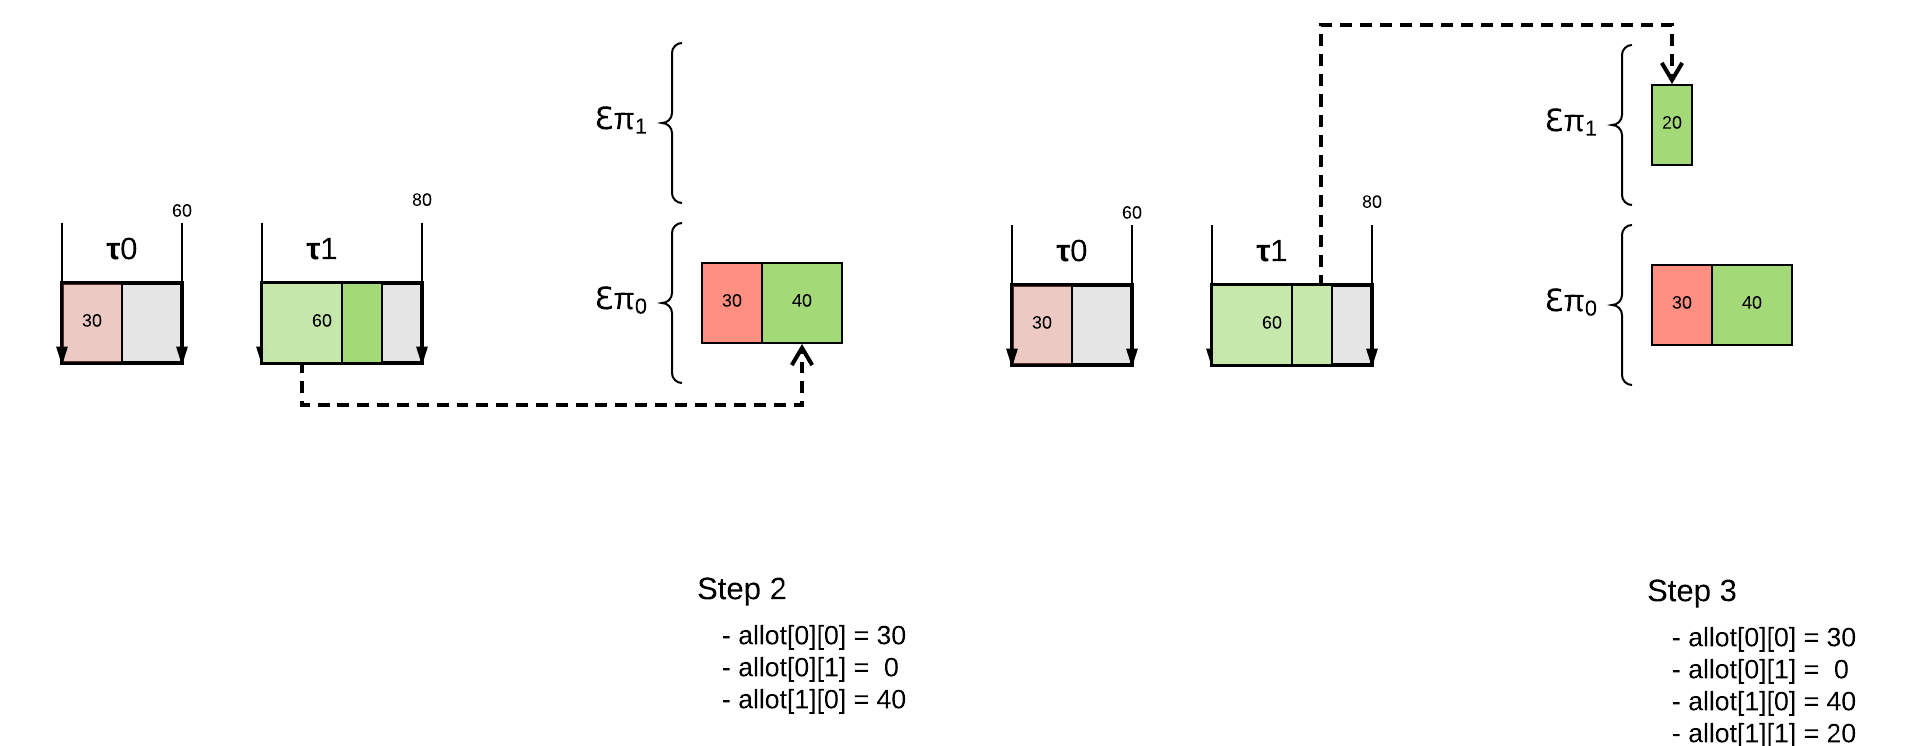
\includegraphics[scale=1]{img/uedf/uedf34}
		\caption{étapes 2 et 3}
	\end{figure}
	\paragraph{Eligible}
	À ce stade, aucune décision d'ordonnancement n'est encore prise, mais des ensembles de tâches (\textit{Eligible}, 
	noté $\epsilon$ dans la suite) sont créés sous forme de listes. Chaque liste \textit{Eligible} définit 
	les seules tâches que les processeurs associés peuvent exécuter (en cela, cette phase d'\textbf{UEDF} peut 
	être considérée comme une phase de partitionnement) durant l'exécution à venir.\newline
	
	Notons que les calculs fournis par l'algorithme permettent en théorie de \og{}remplir\fg{} 
	la charge d'un processeur à 100\% d'utilisation avant de passer au suivant. Concrètement, 
	cela signifie que si la première tâche a une utilisation de moins de 100\%, elle sera suivie par 
	au moins une partie d'une autre.\newline
	
	Les valeurs d'$Allot$ ne doivent pas être considérées comme le temps d'exécution qui sera réellement 
	exécuté sur le processeur. Il faut garder à l'esprit qu'à chaque relâchement de travail, 
	$Allot$ sera recalculé. 

	\paragraph{Prise de décision}
	La phase de décision de l'ordonnancement se déroule lors de la phase suivante.
	\textbf{UEDF} s'inspire pour finir de \textbf{EDF-Delay}. 
	Cet algorithme est très simple :
	\begin{itemize}
		\setlength\itemsep{0.1em}
		\item Une tâche $\tau_i \in \epsilon_j$ est attribuée à un processeur si aucun autre processeur d'index plus bas n'est en train de l'exécuter
		\item $\tau_i$ s'exécute sur le processeur tant qu'$allot_{ij} > 0$.
	\end{itemize}


	\subsubsection{Déroulement}	
	L'algorithme $Compute Allot$ est à effectuer à chaque relâchement de tâche. La valeur $Allot_{ij}$ 
	doit être mise à jour à chaque prise de décision. Une décision est attendue pour chacun des événements suivants :
	\begin{itemize}
		\setlength\itemsep{0.1em}
		\item Une instance de tâche (travail) a été relâchée
		\item Un travail est terminé
		\item $allot{ij} = 0$, pour $i$ un travail et $j$ un processeur 
	\end{itemize}
	
	On peut voir en théorie l'ordonnancement de trois tâches en annexe, afin de mieux comprendre le déroulement d'une exécution.
	À titre de remarque, le travail d'illustration d'une exécution nous semble 
	important pour procéder à une implémentation, sinon le risque est d'omettre le développement 
	d'outils indispensables au bon déroulement de l'exécution. L'algorithme n'est pas évident à mettre en œuvre.
	\todo{gantt chart avec exemple 30;60, 60; 80, 60;80}
	\newline
	
	Nous pouvons déjà formuler ici une nuance par rapport à la théorie et les attentes que l'on peut en avoir 
	en pratique : 
	Nous savons dès le départ que l'algorithme \textbf{UEDF} est assez gourmand en calcul puisque chaque relâchement de 
	tâche va provoquer l'exécution de l'algorithme $Compute Allot$, or, le calcul de cette valeur 
	implique un parcours de toutes les tâches ordonnées, pour chaque processeur. 
	Outre qu'il est nécessaire de gérer une structure de données efficace, nous pouvons 
	déjà considérer que le tri de la structure sera d'un coût non négligeable lors de l'exécution. \newline
	
	Par ailleurs, le calcul même de $Compute Allot$ implique lui aussi une certaine complexité.
	Ainsi :
	\begin{itemize}
		\setlength\itemsep{0.1em}
		\item soit $m$ le nombre de processeurs
		\item soit $n$ le nombre de tâches actives [\ref*{tacheactive}] du système
		\item $Compute Allot \in O(m\times n)$
	\end{itemize}

	Et pour finir, régulièrement, la valeur $allot_{ij} \forall i \in TaskSet, \forall j \in m$ doit être mise 
	à jour, dont la complexité est donc :
	\begin{itemize}
		\setlength\itemsep{0.1em}
			\item soit $m$ le nombre de processeurs
			\item soit $n$ le nombre de tâches actives [\ref*{tacheactive}] du système
			\item $update Allot \in O(m\times n)$
	\end{itemize}

	Nous pouvons attendre un surcoût important sur cette base. Une hypothèse étant que ce surcoût 
	augmente avec le nombre de tâches, mais aussi avec le nombre de cœurs. Un même système pourrait avoir plus 
	de surcoût avec plus de cœurs. Cela pourra être vérifié dans les expérimentations.

	\newpage
	
	
	
	
	
	
	
	
	
	
	
	
	
	
	
	
	
	\subsection{Comparaison avec Global-EDF}
	
	Nous avons choisi de comparer \textbf{UEDF} à \textbf{Global-EDF} [\ref*{GlobalEDF}]. 
	La raison de ce choix est simple : 
	cet algorithme est implémenté sur le RTOS HIPPEROS et il est global, comme 
	l'indique son nom. 
	Les autres ordonnanceurs disponibles sur HIPPEROS sont pour la plupart partitionnés.
 
	Aussi les tests effectués sur \textbf{UEDF} seront également faits en utilisant \textbf{Global-EDF} pour 
	élément de comparaison.\newline
	
	Ces deux algorithmes ont toutefois de grandes différences. \textbf{Global-EDF}
	ne permet pas - même théoriquement  d'atteindre l'optimalité. Ceci s'explique par le fait que 
	\textbf{Global-ED}F peut être considéré comme \og{}vertical\fg{} là où \textbf{UEDF} serait \og{}horizontal\fg{}. 
	Mais une grande différence entre les deux algorithmes est que \textbf{Global-EDF} n'a pas de clairvoyance, 
	et n'est par conséquent pas optimal, même en théorie, pour la classe périodique, 
	contrairement à \textbf{UEDF}.
	
	\subsubsection{Fonctionnement de Global EDF}
	
	L'algorithme est relativement simple, et pour les besoins de la comparaison, nous résumons 
	ici son fonctionnement.\\
	À un moment \textit{t}, l'ordonnanceur prend sa décision de cette façon :
	si un processeur est libre, il se voit attribué le travail de priorité supérieure parmi 
	tous les travaux actifs. Cela permet d'avoir un algorithme peu gourmand.
	
	\begin{algorithm}
	\caption{Global-EDF}
	\begin{algorithmic}
		\REQUIRE $JobSet(t)$ ordonné par échéances
		\FORALL{ $j \in m $}
			\item $decision \leftarrow pop(JobSet(t))$
		\ENDFOR
	\end{algorithmic}
\end{algorithm}	
	
	L'algorithme permet de prendre une décision au moment \textit{t} en ne considérant 
	que les travaux à exécuter par ordre de priorité et les processeurs disponibles.
	
	Si l'on reprend l'exemple illustré précédemment, la décision sera prise de cette façon :z
	
	\begin{figure}[H]
		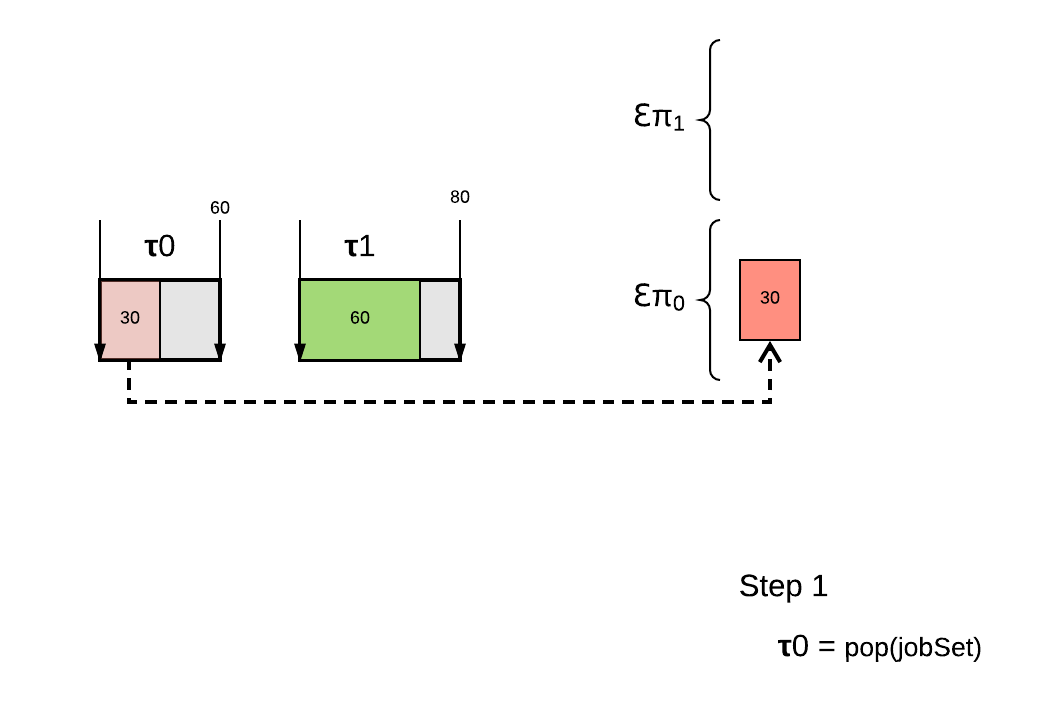
\includegraphics[scale=0.5]{img/gedf/gedf}
		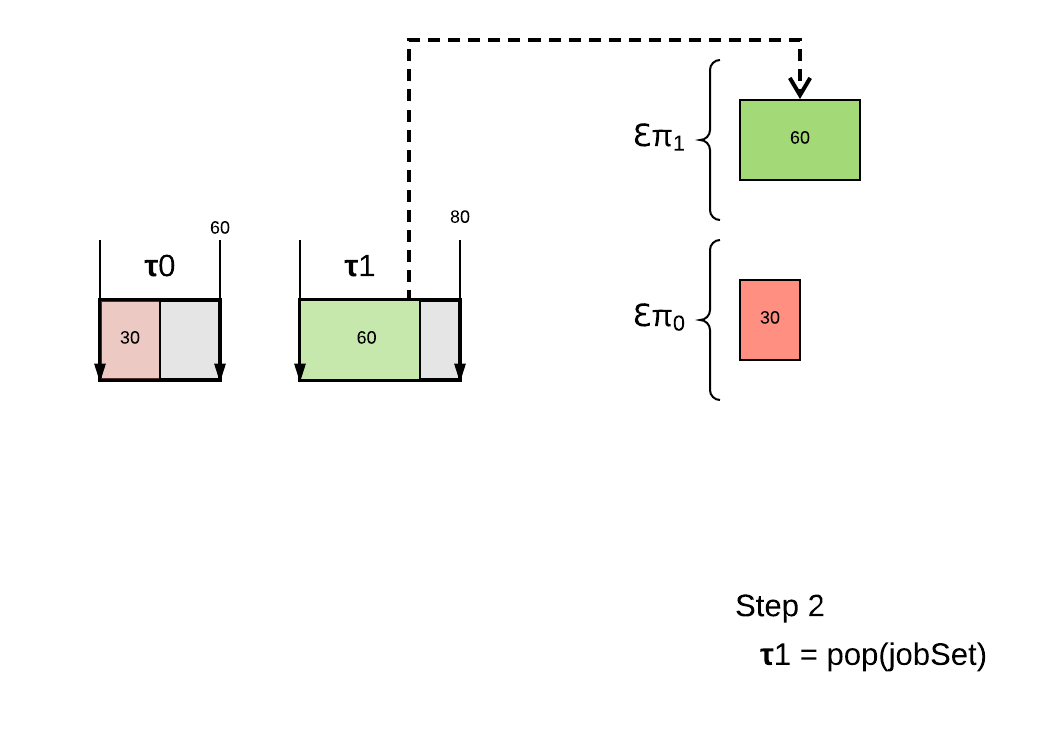
\includegraphics[scale=0.5]{img/gedf/gedf2}
		\caption{Global EDF}
	\end{figure}
	 
	On peut facilement voir que cela peut entraîner de \og{}mauvais choix\fg{}. 
	En changeant l'exemple précédent, et en prenant un exemple avec 3 travaux, 
	on n'obtiendra pas du tout le même ordonnancement dans les deux algorithmes, 
	et celui-ci mettra en échec \textbf{Global-EDF} quasiment immédiatement.\newline
	
	Prenons un ensemble de trois tâches comme suit :

	\begin{enumerate}
		\setlength\itemsep{0.1em}
		\item $\tau_1 : \{o:0; w:40; d=p:60;\}$
		\item $\tau_2 : \{o:0; w:40; d=p:60;\}$
		\item $\tau_3 : \{o:0; w:40; d=p:60;\}$
	\end{enumerate}
	
	\todo{insérer schema ici}
	
	Malgré ce point, \textbf{Global-EDF} est \og{}efficace\fg{} en terme de calculs.
	Le point le plus complexe concerne la structure de données qui conserve les 
	tâches courantes. Une bonne idée est d'utiliser un Heap [\ref*{heap}] qui 
	va permettre de fournir toujours en tête le travail de priorité supérieure.
	Pour s'assurer de la faisabilité de l'ensemble de tâches, 
	il faudra tester l'ordonnancement suffisamment longtemps (hyper-période).\newline

		
\section{HIPPEROS}
	\customhighlight{HIPPEROS} (\textbf{HI}gh \textbf{P}erformance \textbf{P}arallel \textbf{E}mbedded \textbf{R}eal-time \textbf{O}perating \textbf{S}ystems)
	est un \customhighlight{RTOS} (Real-Time Operating System) développé depuis plusieurs années par une spinoff de l'ULB.
	Il bénéficie des connaissances apportées par le monde de la recherche dans 
	le domaine des systèmes critiques avec multic\oe{}urs. Une de ses particularités 
	est sa modularité, qui permet d'adapter ses possibilités en fonction du système 
	lors de la compilation de l'OS, ainsi peut-on différencier principalement 
	deux installations en fonction des particularités. 
	
	\customhighlight{HIPPEROS} est un candidat idéal pour l'implémentation d'un ordonnanceur 
	global. Il a cependant un fonctionnement propre qui pourra rendre l'implémentation 
	plus ou moins facile, et poser un certain nombre de problèmes. 
	En résumé, une nouvelle implémentation sur un OS différent 
	peut elle-aussi apporter à la connaissance générale des détails importants.
		
\section{Attentes}

	Des présentations des différents acteurs qui ont été faites dans les parties précédentes, à savoir :
	\begin{enumerate}
		\setlength\itemsep{0.1em}
		\item UEDF
		\item Global-EDF
		\item HIPPEROS
	\end{enumerate}
	nous pouvons déjà formuler certaines hypothèses que nous aimerions vérifier dans ce travail. \newline
	Il est important de mesurer les surcoûts liés à l'algorithme \textbf{UEDF}, car il n'est pas 
	évident en voyant l'algorithme qu'il soit possible de l'utiliser en pratique. \newline
	Il serait intéressant de mesurer également si l'on observe bien en pratique que Global-EDF ne 
	peut pas ordonnancer certains systèmes là où UEDF le pourrait. En raison des surcoûts, encore, il 
	se pourrait qu'en moyenne, ce résultat soit modifié ou largement à nuancer en 
	fonction de certains paramètres, comme le WCET, dont nous reparlerons.
	Il serait intéressant également de comparer le nombre de migrations/préemptions 
	obtenues pour le même système, ordonnancé par l'un ou par l'autre des algorithmes.

